\chapter*{Введение} % * не проставляет номер
\addcontentsline{toc}{chapter}{Введение} % вносим в содержание

В этой работе исследуется совместная работа нескольких агентов с использованием алгоритмов и методов глубокого обучения в 2D игровых средах. Имея это в виду, мы изучили и адаптировали современные алгоритмы и методы обучения глубокого обучения с подкреплением к настройкам игры с несколькими агентами.

Глубокое обучение с подкреплением - это новая область исследований алгоритмов и методов, которая сочетает в себе обучение с подкреплением и глубокое обучение. Предыдущие работы в основном были направлены на адаптацию глубоких нейронных сетей для усиления алгоритмов обучения. Например, глубокая Q-сеть (Deep Q-network, DQN) \cite{Mnih2015} интегрирует глубокие нейронные сети в Q-обучение, классический табличный алгоритм обучения с подкреплением. Обученные сети могут играть в различные игры Atari 2600 \cite{Bellemare_2013} лучше человека. Это считается первой успешной попыткой научиться играть в видеоигры с прямым визуальным вводом большого размера. Алгоритм глубокого детерминированного градиента политики (deep deterministic policy gradient, DDPG) \cite{lillicrap2015continuous} является еще одним примером использования глубоких нейронных сетей в контексте обучения с подкреплением и непрерывного пространства действий.

Большинство исследований посвящено обучению одного агента. Однако проблемы, связанные с мультиагентным сотрудничеством или конкуренцией, также очень распространены в социальной, экономической и инженерной областях. Игры представляют собой упрощенные версии реальных задач, которые можно сделать идеальными тестовыми площадками для экспериментов. Поэтому в этой работе игровые сценарии используются для изучения алгоритмов глубокого обучения с подкреплением для совместной работы нескольких агентов.

\section{Вопросы исследования} \label{intro:sec1}

В этой работе мы исследуем следующие вопросы:
\begin{enumerate}[1.]
	\item Как несколько агентов могут научиться сотрудничать друг с другом во время обучения в определенных игровых сценариях?
	\item Может ли после обучения появиться язык между агентами в определенных игровых сценариях?
	\item Как можно оптимизировать и ускорить процесс обучения?
\end{enumerate}
Сначала мы изучим современные алгоритмы и методы глубокого обучения с подкреплением. Затем мы проведем эксперименты игровых сценариев в модифицированной среде от компании OpenAI \cite{OpenAI-Gym}. Наконец, мы рассмотрим и применим различные приемы для оптимизации процесса обучения.

\section{Сценарии} \label{intro:sec2}

Чтобы исследовать вышеизложенные вопросы, мы используем несколько сценариев, где агенты общаются друг с другом и физически перемещаются к определенным целям. Некоторые из сценариев являются точными копиями экспериментов, проведенных в недавней работе \cite{lowe2017multiagent}, а другие представляют собой новые сценарии, которые расширяют исходные с целью дальнейшего изучения многоагентного сотрудничества и коммуникации.

\subsection{Сценарий 1: Simple Speaker Listener} \label{intro:ssl}

В этом сценарии есть три ориентира, представленные как красные, зеленые и синие ориентиры, как показано на рисунке. Два агента с разными функциями должны сотрудничать для достижения общей цели. \textit{Говорун} (серый агент) не может двигаться, но видит цвет цели и может говорить с другим агентом. \textit{Слушатель} (отображаемый таким же цветом, что и его цель) видит все ориентиры и их цвета (но не видит собственный цвет, т.е. не знает, какой из объектов является его целью), а так же слышит \textit{говоруна} и пытается перейти к правильному ориентиру. Более подробные настройки среды этого сценария можно найти в разделе \hyperref[ch4:exp-ssl]{4,1}.
% TODO хардкод номера главы

\begin{figure}[ht!] 
	\center
	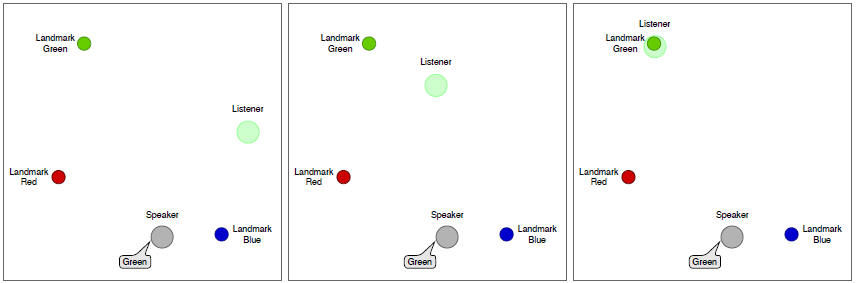
\includegraphics [scale=0.80] {my_folder/images/fig0-1-simple-speaker-listener.png}
	\caption{Сценарий 1. \textit{Simple Speaker Listener}. Скриншоты слева направо показывают этапы игрового эпизода. \textit{Говорун} (серый) выдает коммуникационное действие, представляющее «зеленый», а \textit{слушатель}, слушает сообщение \textit{говоруна} и направляется к цели.} 
	\label{fig:0-1-simple-speaker-listener}  
\end{figure}

\begin{figure}[ht!] 
	\center
	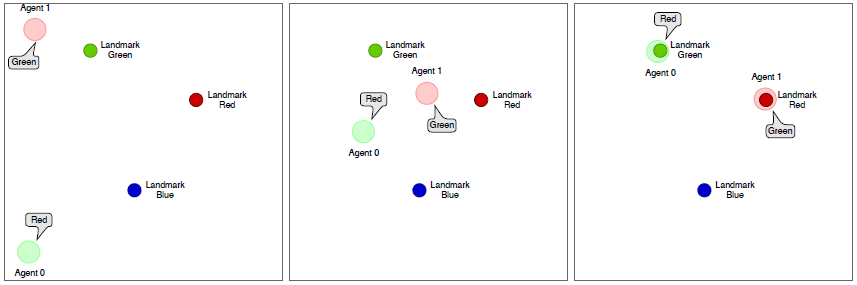
\includegraphics [scale=0.80] {my_folder/images/fig0-2-simple-reference.png}
	\caption{Сценарий 2: \textit{Simple Reference}. В этом эпизоде агент 0 (отображаемый в том же цвете, что и его целевой ориентир) выдает коммуникационное действие, представляющее «красный», и слушает агента 1. А агент 1 (отображается в том же цвете, что и его целевой ориентир), слушает и издает «зеленый» для Агента 0. Скриншоты слева направо показывают, как ведут себя два агента в соответствии с оптимальными политиками, слушая друг друга и перемещаясь к целям.} 
	\label{fig:0-1-simple-reference}  
\end{figure}

\subsection{Сценарий 2: Simple Reference}

Этот сценарий расширяет предыдущий, поскольку оба агента являются одновременно и \textit{говорунами} и \textit{слушателями}. Ориентиры остаются прежними, отображаются как три разноцветных объекта, (как изображено на \firef{fig:0-1-simple-reference}). Каждый из двух агентов пытается достичь своего целевого ориентира, который известен только другому агенту. Таким образом, он должен научиться сообщать другому агенту его цель и перемещаться к своей собственной. Что отличает сценарий от двух копий сценария \textit{Simple Speaker Listener}, так это то, что единое общее вознаграждение, присуждаемое агентам, основано на общей производительности. Таким образом, агенты должны выяснить, что идет хорошо, а что нет. Настройка среды подробно описана в разделе Х.Х.
% TODO добавить ссылку на другой раздел

\section{Практическая значимость} \label{intro:sec3}

Проект сосредоточен на обучении нескольких агентов совместной работе с использованием глубокого обучения в игровой среде. Результаты исследования могут быть дополнительно разработаны и широко использованы во многих практических реальных приложениях в области экономики, управления, техники и т. д. Например, он может применяться в робототехнике, к автономным транспортным средствам, производственным линиям, фондовым рынкам и т. д.

Перед применением в этих областях, алгоритмы и методы, которые исследуются и разрабатываются в этой работе, должны быть хорошо протестированы и проверены, поскольку эти приложения непосредственно влияют на безопасность человека, социальную и финансовую безопасность. В долгосрочной перспективе применение мультиагентных алгоритмов приведет к появлению все большего числа автономных систем во многих областях. 


%% Вспомогательные команды - Additional commands
%\newpage % принудительное начало с новой страницы, использовать только в конце раздела
%\clearpage % осуществляется пакетом <<placeins>> в пределах секций
%\newpage\leavevmode\thispagestyle{empty}\newpage % 100 % начало новой строки
